\documentclass[12pt]{article}
\usepackage[utf8]{inputenc}
\usepackage{amsmath, amssymb, amsthm, graphicx, fancyvrb, enumitem, titlesec, setspace, float, fancyvrb, minted}
\usepackage[dvipsnames]{xcolor}
\usepackage[top=1in, bottom=1in, left=1.25in, right=1.25in]{geometry}
\titleformat{\section}{\normalfont\bfseries}{}{0em}{}
\titlespacing*{\section}{0pt}{1.5ex plus .2ex minus .2ex}{0.8ex plus .1ex}


\begin{document}
\noindent Andre Winkel \hfill \today \\
\rule{\textwidth}{0.4pt} \vspace{0em}
\begin{center} \large{Lab 3} \end{center} \vspace*{0em}

\section*{Problem 1: Evaluating stability of second order systems}
In this problem, we will evaluate the stability of LTI systems described by a second order difference equation.
\begin{enumerate}[label=\textbf{\alph*)}, leftmargin=2.6em]

\item From the provided block diagram, we can infer that the difference equation must be
\begin{equation}
    x[n]=y[n]-y[n-1]+c_0y[n-2].
\end{equation}

\item If we allow $x[n]=u[n-10]$ and $c_0=0.2$, we can evaluate the output $y[n]$ recursively. The output, $y[n]$, is plotted below for $n=0,1,2,...,200$:
\begin{figure}[H]
    \centering
    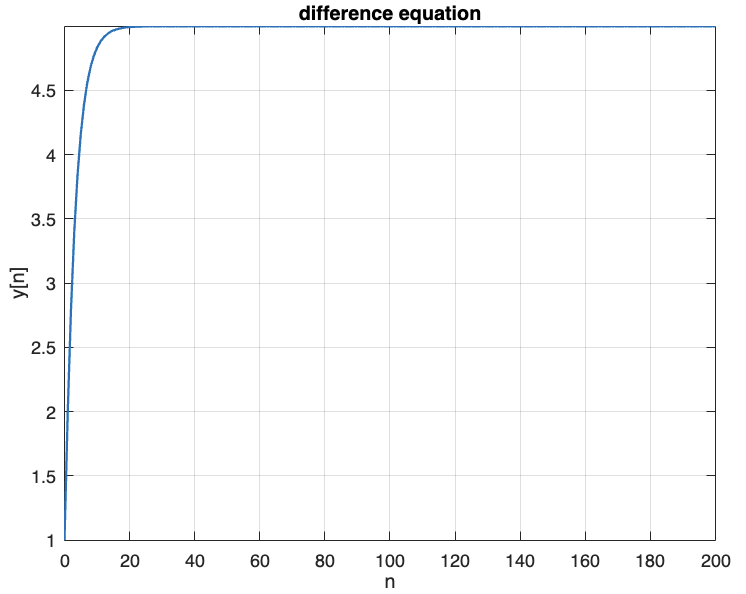
\includegraphics[width=0.5\linewidth]{plot1.png}
\end{figure}
\begin{minted}[frame=single, fontsize=\small, linenos, bgcolor=white]{matlab}
% The next two lines make your plots look better
set (0, 'DefaultAxesFontSize', 12) ;
set (0, 'DefaultLineLineWidth', 1.5) ;
n_arr = 0:200;
c_0 = 0.2;
x_arr = ones (1, length(n_arr));
y_arr = zeros (1 , length(n_arr)) ;

for idx = 1: length ( n_arr )
    if idx == 1
        y_arr(idx) = x_arr(idx);
    elseif idx == 2
        y_arr(idx) = x_arr(idx) + y_arr(idx - 1);
    else
        y_arr(idx) = x_arr(idx) + y_arr(idx - 1) - c_0*y_arr(idx-2);
    end
end

plot (n_arr , y_arr);
title('difference equation', 'FontSize', 16)
xlabel('n', 'FontSize', 16);
ylabel('y[n]', 'FontSize', 16);

%% The next two lines make your plot look better
axis tight ;
grid on;
\end{minted}

\item Repeating part (a) with $c_0=0.7$, $c_0=0.9$, and $c_0=1.1$, we observe the following plots:
\begin{figure}[H]
    \centering
    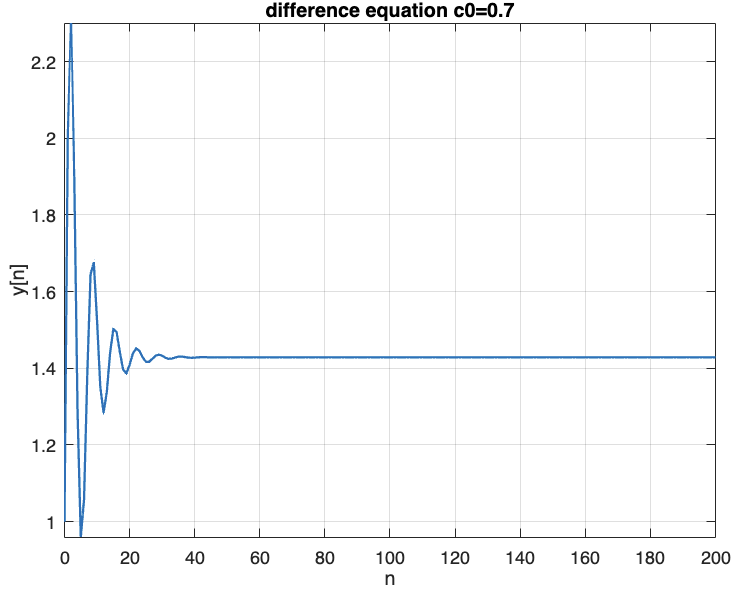
\includegraphics[width=0.32\linewidth]{plot2.png}
    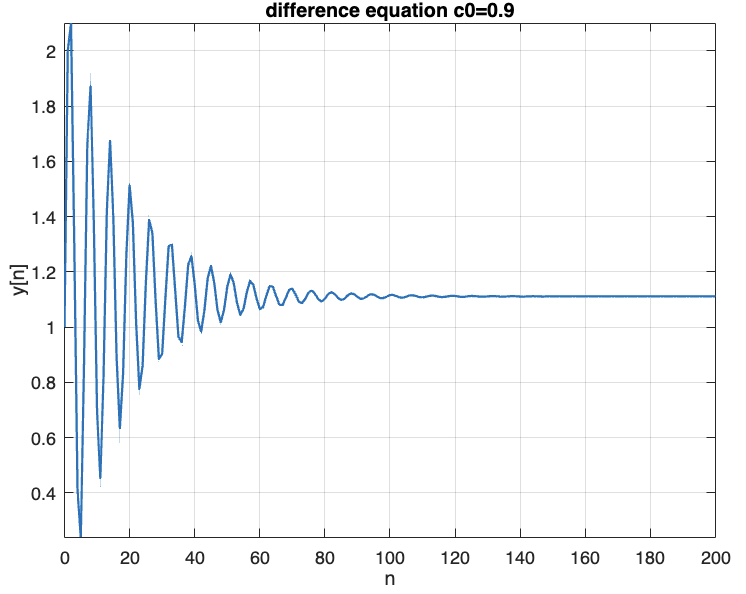
\includegraphics[width=0.32\linewidth]{plot3.png}
    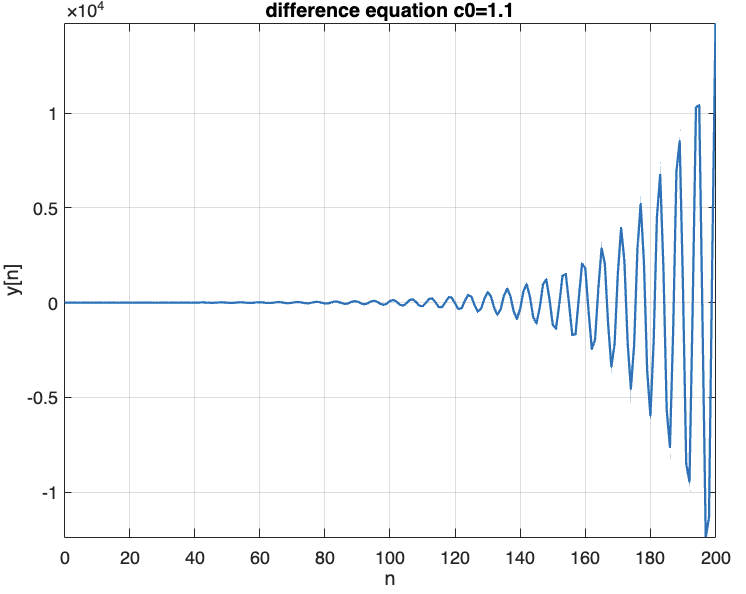
\includegraphics[width=0.32\linewidth]{plot4.png}
\end{figure}
We can directly observe that when $c_0<1$, the plots of $y[n]$ oscillate before damping to convergence as $n \to \infty$, more accurately described by $\lim_{n \to \infty}y[n]=0$. On the other hand, the plot of $y[n]$ with $c_0=1.1$ begins at stability before oscillating to divergence as $n$ increases, analogous to $\lim_{n \to \infty}y[n]=\infty$. We are also able to directly observe that as we increase the value of $c_0$, the maximum value within the plotted range decreases.

\item Repeating this process for $c_0=0.2,0.7,0.9,1.1$ and with $x[n]=\cos[\frac{\pi n}{3}]$, we observe the following plots:
\begin{figure}[H]
    \centering
    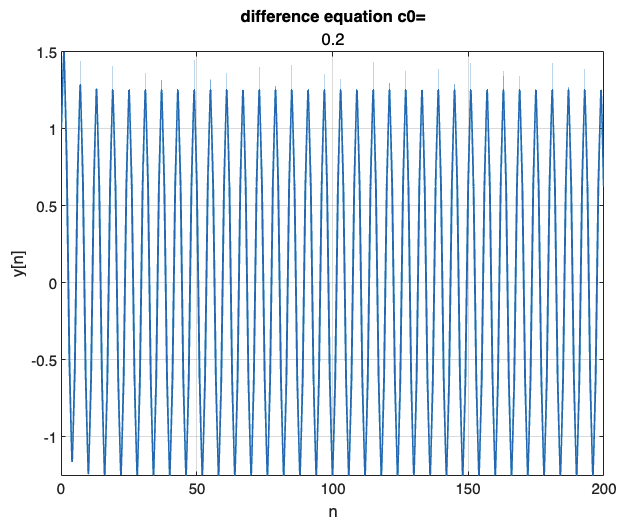
\includegraphics[width=0.49\linewidth]{plot5.png}
    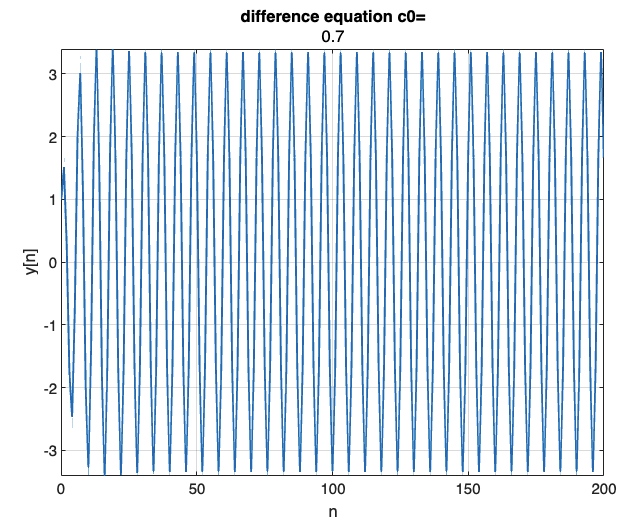
\includegraphics[width=0.49\linewidth]{plot6.png}
    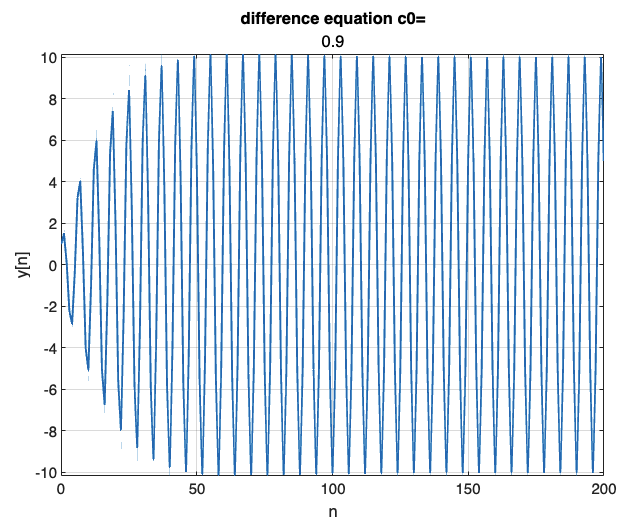
\includegraphics[width=0.49\linewidth]{plot7.png}
    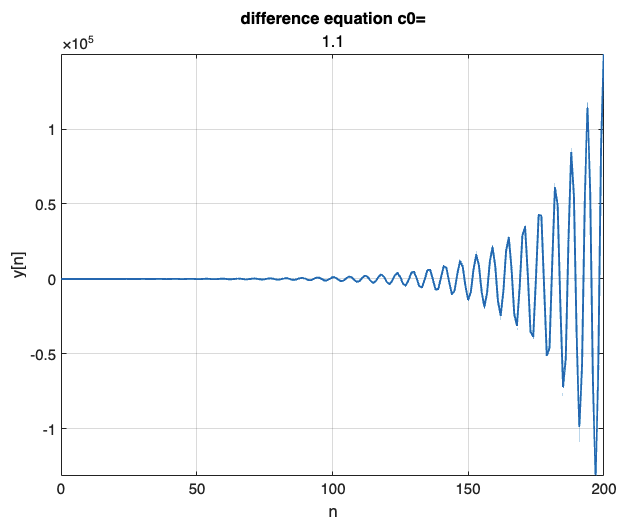
\includegraphics[width=0.49\linewidth]{plot8.png}
\end{figure}
\begin{minted}[frame=single, fontsize=\small, linenos, bgcolor=white]{matlab}
% The next two lines make your plots look better
set (0, 'DefaultAxesFontSize', 12) ;
set (0, 'DefaultLineLineWidth', 1.5) ;
n_arr = 0:200;
c_0 = 1.1;

x_arr = cos(pi .* n_arr / 3);

y_arr = zeros (1 , length(n_arr)) ;

for idx = 1: length ( n_arr )
    if idx == 1
        y_arr(idx) = x_arr(idx);
    elseif idx == 2
        y_arr(idx) = x_arr(idx) + y_arr(idx - 1);
    else
        y_arr(idx) = x_arr(idx) + y_arr(idx - 1) - c_0*y_arr(idx-2);
    end
end

% You can use stem here , but it will be difficult to understand .
plot (n_arr , y_arr );
title('difference equation c0=', c_0, 'FontSize', 16)
xlabel('n', 'FontSize', 16);
ylabel('y[n]', 'FontSize', 16);

%% The next two lines make your plot look better
axis tight ;
grid on;
\end{minted}
We see here that the amplitude of $y[n]$ increases with an increased $c_0$. Furthermore, we observe that when $c_0=1.1$, $y[n]$ becomes unbounded as $n\to\infty$, with its amplitude also approaching $\infty$.

\item In this part, we will create an array for $w_0$ and repeat the procedure with $x[n]=cos(\omega_0n)$, with $c_0=0.8$. The plot of $y_{\text{max}}(\omega_0)$ versus $\omega_0$ is shown below:
\begin{figure}[H]
    \centering
    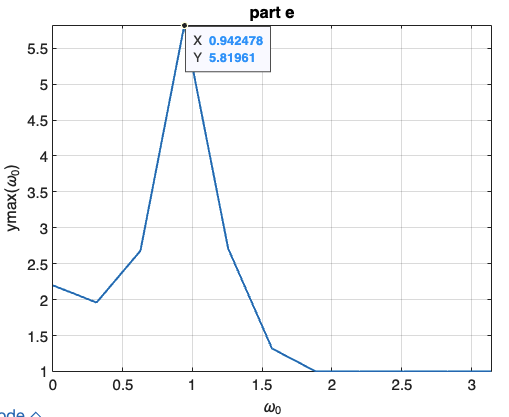
\includegraphics[width=0.5\linewidth]{plot9.png}
\end{figure}
\begin{minted}[frame=single, fontsize=\small, linenos, bgcolor=white]{matlab}
% The next two lines make your plots look better
set (0, 'DefaultAxesFontSize', 12) ;
set (0, 'DefaultLineLineWidth', 1.5) ;
n_arr = 0:200;
c_0 = 0.8;

x_arr = cos(pi .* n_arr / 3);
y_arr = zeros (1 , length(n_arr));
omega_0_arr = linspace(0, 1, 11)*pi;
max_arr = zeros(1, length(omega_0_arr));

for m_idx = 1:length(omega_0_arr)
    x_arr = cos (n_arr*omega_0_arr(m_idx)) ;
    y_arr = zeros (1, length(n_arr)) 
    for idx = 1:length(n_arr)
        if idx == 1
            y_arr(idx) = x_arr(idx);
        elseif idx == 2
            y_arr(idx) = x_arr(idx) + y_arr(idx - 1);
        else
            y_arr(idx) = x_arr(idx) + y_arr(idx - 1) -
            c_0*y_arr(idx-2);
        end
    end
    max_arr(m_idx) = max(y_arr);
end

% You can use stem here , but it will be difficult to understand .
plot (omega_0_arr, max_arr);
title('part e', 'FontSize', 16)
xlabel('\omega_0', 'FontSize', 16);
ylabel('ymax(\omega_0)', 'FontSize', 16);

%% The next two lines make your plot look better
axis tight ;
grid on;
\end{minted}
Here, we can observe that the peak of $y_{\text{max}}(\omega_0)$ is at $\omega_0\approx0.942$.

\end{enumerate}
\end{document}